
\section{Random Forest}

In this section we will be discussing the \textit{Random Forest} algorithm. As mentioned previously, a Random Forest is an ensemble 
of individual decision trees trained via the bagging or pasting method (Mostly bagging). In Scikit-Learn, there are both 
\mintinline{python}{RandomForestClassifier} and \mintinline{python}{RandomForestRegressor} depending on the task we need to complete at 
hand. \\

\noindent
The code below will train a Random Forest classifier with 500 trees using all available CPU cores (Each tree limited to 16 nodes):

\begin{minted}{python}
from sklearn.datasets import make_moons
from sklearn.model_selection import train_test_split
from sklearn.ensemble import RandomForestClassifier

X, y = make_moons(n_samples=500, noise=0.30)
X_train, X_test, y_train, y_test = train_test_split(X, y)

rnd_clf = RandomForestClassifier(n_estimators=500, max_leaf_nodes=16, 
                                 n_jobs=-1)
rnd_clf.fit(X_train, y_train)

y_pred_rf = rnd_clf.predict(X_test)
\end{minted}

\noindent
For the most part a \mintinline{python}{RandomForestClassifier} has all the hyperparameters of a \mintinline{python}{DecisionTreeClassifier}
(to control how the trees are grown), plus the ability to control the ensemble of the trees as well. \\

\noindent
The Random Forest Algorithm introduces more randomness when growing trees; instead of searching for the very best feature when splitting
a node, it searches for the best feature among a random subset of features. Therefore the algorithm results in greater tree diversity, 
which trades a higher bias for a lower variance, generally returning a overall better model. 

\subsection{Feature Importance}

Conveniently, Random Forests are also able to make it easy to measure the relative importance of each feature given a dataset. Scikit-Learn
measures a feature's important by looking how much the tree nodes that use the feature reduce impurity on average (across all trees in the
forest). More specifically, it is a weighted averafe, where each node's weight is equal to the number of training samples that are 
associated with it. \\

\noindent
Scikit-Learn computes the score automatically and then scales the result fo that the sum of all feature importances are equal to 1. To 
access these results is fairly straight forward by calling the \mintinline{python}{feature_importances_} variable. For example, below 
will be a code block trainig a \mintinline{python}{RandomForestClassifier} on the iris dataset and outputs each feature's importance.\\

\begin{minted}{python}
from sklearn.datasets import load_iris

iris = load_iris()
rnd_clf = RandomForestClassifier(n_estimators=500, njobs=-1)
rnd_clf.fit(iris["data"], iris["target"])

for name,score in zip(iris["feature_names"], rnd_clf.feature_importances_):
    print(name, score)

'''
Output:

sepal length (cm) 0.112492250999
sepal width (cm) 0.0231192882825
petal length (cm) 0.441030464364
petal width (cm) 0.423357996355
'''
\end{minted}

\noindent
Now we can see that it seems that the most important features are petal length and petal width with 44\% and 42\% important, respectively.

%In this section we will be discussing how we can combine a group of predictors to generate better predictions. This is commonly known as an 
%\textit{ensemble} which is then extended into \textit{Ensemble Learning}. Some of the most popular Ensemble Methods are \textit{bagging},
%\textit{boosting}, and \textit{stacking}. Additionally, \textit{Random Forests} will also be explained in more detail in this section.

%\subsection{Voting Classifiers}

%Suppose that we have trained a few classifiers, each one acheiving roughly 80\% accuracy (See figure below).

%\begin{center}
%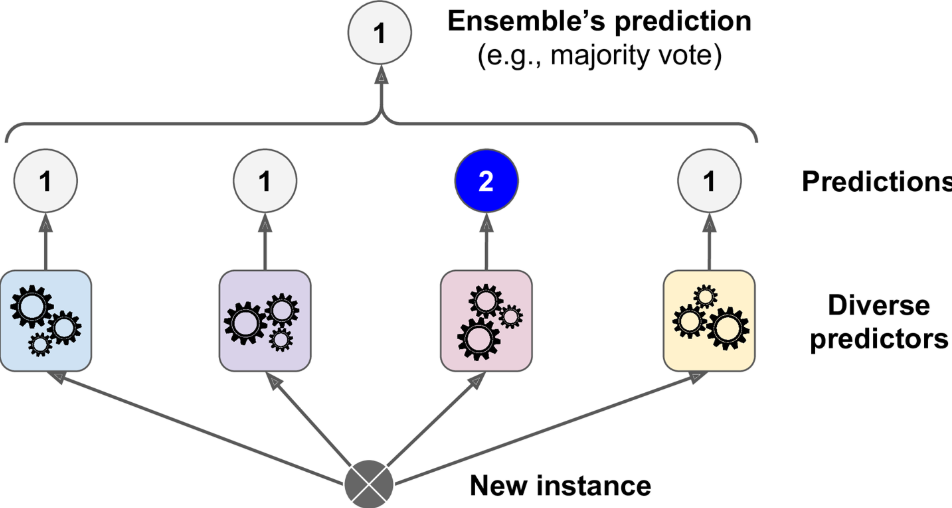
\includegraphics[scale=0.70]{Images/voting_classifier.PNG}
%\end{center}



%\subsection{Bagging and Pasting}

%\subsection{Boosting}

%\subsection{Stacking}